\documentclass[12pt]{article}
\usepackage[brazil]{babel}
\usepackage{graphicx}
\usepackage{mathtools}
\usepackage{float} 
\usepackage{xcolor}


\usepackage{array}
\usepackage{booktabs}



% margenes
\usepackage[a4paper,left=2cm,right=2cm,top=1cm]{geometry}

%opening
\title{\textbf{Programação Científica para Engenharia e Ciência Térmicas \\Lista de Exercícios No. 8}}

\author{Cristian Herledy López Lara}
\date{Junho 2025}

\begin{document}
	
\maketitle


\section*{Questão 4}

Interprete os resultados observados: há tendência clara? Como o aumento de WC afeta a perda de carga? \\


\textbf{\underline{Desenvolvimento}}

Para a interpretação dos resultados, foram selecionados três gráficos para analisar valores baixos, médios e altos de $jg$.

\begin{figure}[H]
	\centering
	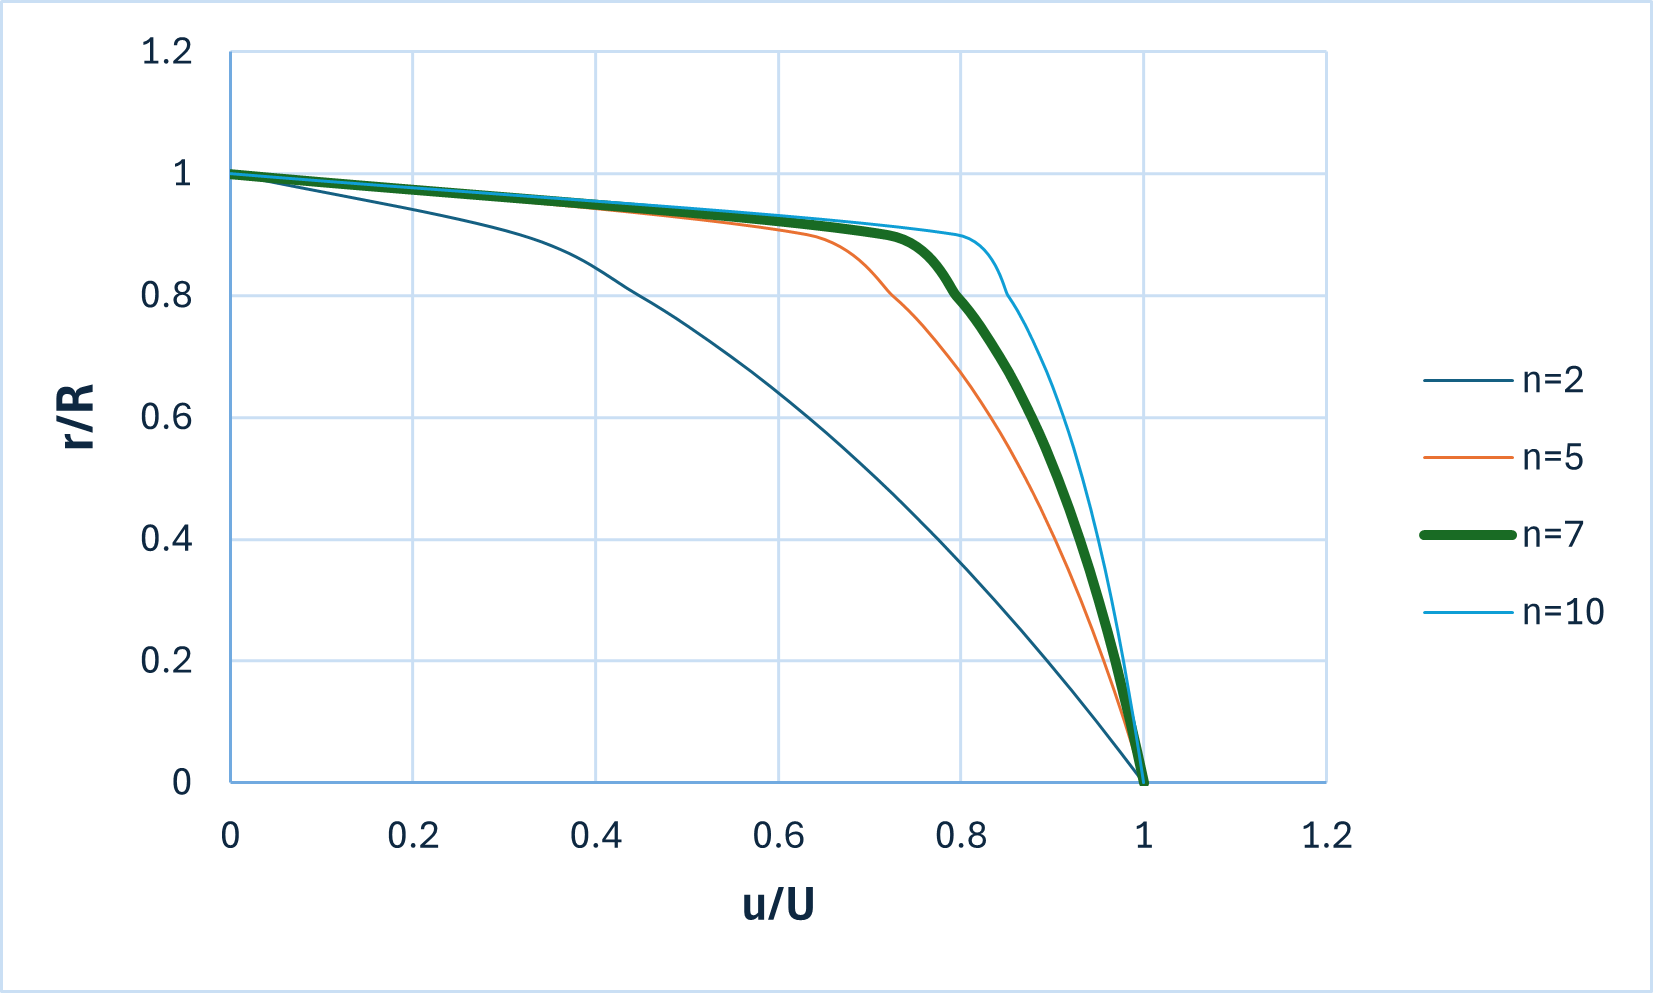
\includegraphics[width=.65\textwidth]{figures/1}
	\caption{Medições perda de carga vs water cut para $V_{sup}$ de 1 m/s}
\end{figure}

Quando o $jg$ é baixo, a perda de carga já é alta desde o início, e o aumento do Water Cut não muda muito isso. Então colocar mais água não afeta tanto a restricão pelo atrito.

\begin{figure}[H]
	\centering
	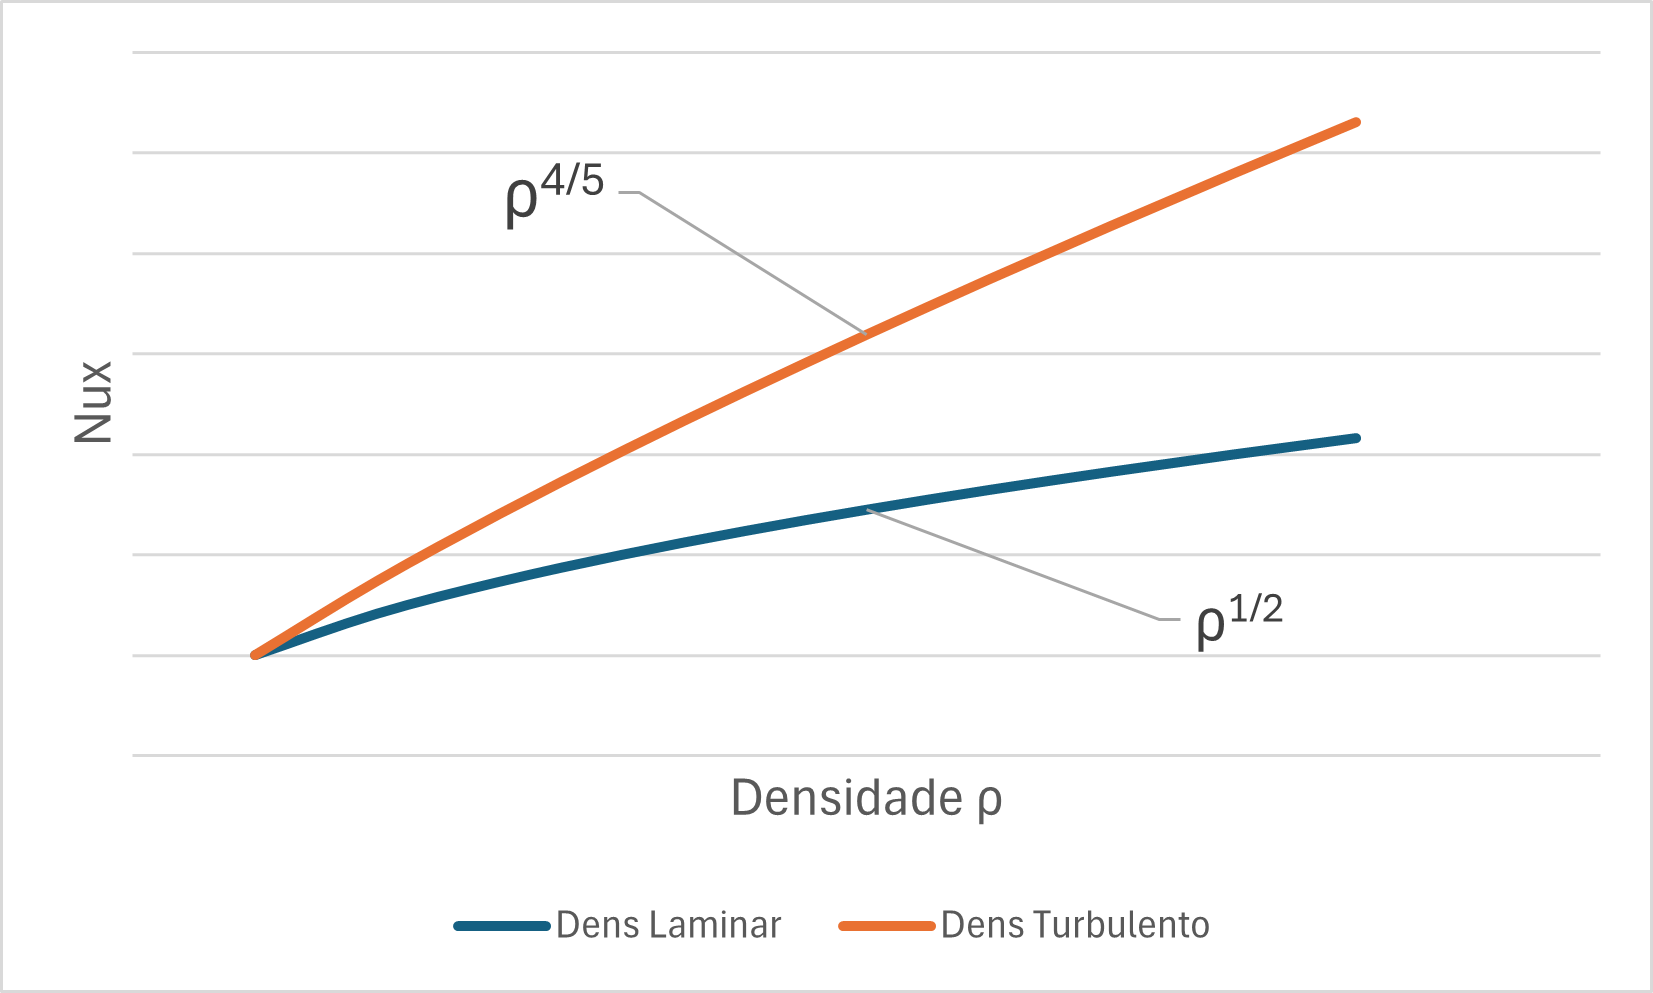
\includegraphics[width=.65\textwidth]{figures/3}
	\caption{Medições perda de carga vs water cut para $V_{sup}$ de 3.5 m/s}
\end{figure}

Em valores médios de jg (perto de 4 $m/s$), é percibido que quando começa a colocar mais água, a perda de carga até diminui um pouco no começo, depois pode subir de novo. Isso pode ser porque o tipo de escoamento muda e fica mais misturado. É importante ressaltar que foram encontrados no arquivo valores negativos de perda de carga por atrito para esta inversão, revelando possíveis erros de medição.


\begin{figure}[H]
	\centering
	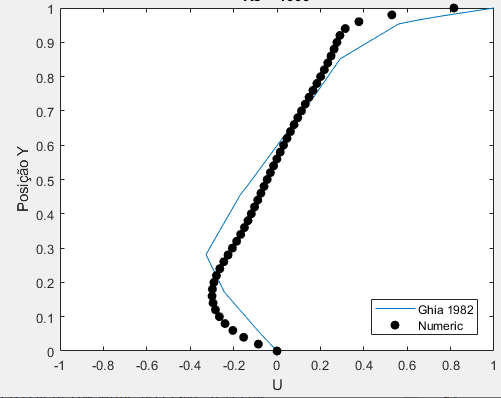
\includegraphics[width=.65\textwidth]{figures/6}
	\caption{Medições perda de carga vs water cut para $V_{sup}$ de 18.5 m/s}
\end{figure}


Para valores elevados de jg, a perda de carga aumenta novamente com o WC, indicando que o aumento do conteúdo de água contribui com o aumento do atrito ao longo do escoamento.

\begin{thebibliography}{999}
	
	
	\bibitem{IFE}
	Morten Langsholt,
	TP/IFE/007: THREEPLEX WP4 – Fluid properties and
	two-phase fluid characterisation experiments.
	Halden, Norway,
	2004.
	
	
	
\end{thebibliography}


\end{document}





